\section{实验结果与分析}

本章节将展示实验结果,并对实验结果进行分析。

\subsection{实验结果}

编写完成所有函数之后,在\texttt{proj5.ipynb}中对光学神经网络模型在MNIST数据集上进行训练和测试。其中batch size为64,学习率为0.00001,训练轮数为30。图\ref{fig:loss_and_acc}展示了训练过程中的损失和准确率变化。

\begin{figure}[H]
    \centering
    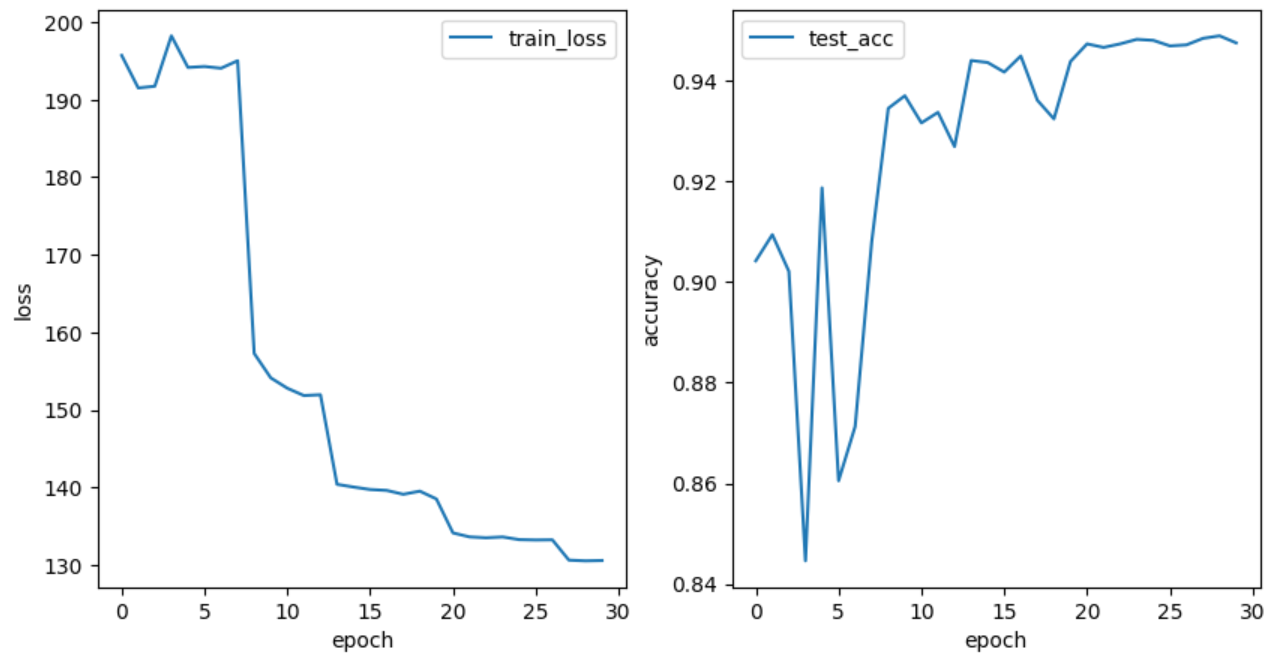
\includegraphics[width=0.95\textwidth]{pics/loss_and_acc.png}
    \caption{训练过程中的损失和准确率变化}
    \label{fig:loss_and_acc}
\end{figure}

如图所示,模型在训练过程中损失逐渐下降,准确率逐渐上升。在训练结束时,模型的准确率达到了94.9\%,完成了对光学神经网络模型的训练过程。

\subsection{实验分析}

光学神经网络是一种基于光学器件的神经网络模型,可以实现对光学信号的处理。为了训练和测试光学神经网络模型,通常在计算机上进行模拟。本次实验搭建了一个简单的光学神经网络模型,将图像转换到频域进行处理,然后再转换回空间域。本实验中的光学神经网络的代码如下所示:

\begin{lstlisting}[style=Python]
class onn(nn.Module):
    def __init__(self):
        super(onn, self).__init__()
        self.height_map_var = torch.randn([otf_size, otf_size, 1, 1])
        self.height_map_var = self.height_map_var.div(1000)
        self.height_map_var = nn.Parameter(self.height_map_var)
        self.refractive_index = 1.5
        self.delta_N = self.refractive_index - 1.000277
        self.wave_lengths = 550e-9
        self.wave_nos = 2. * np.pi / self.wave_lengths

    def forward(self, x):
        height_map = torch.square(self.height_map_var)
        phi = self.wave_nos * self.delta_N * height_map
        phase_shifts = commplex_exp_torch(phi)
        atf = phase_shifts

        x = torch.reshape(x, [-1, 32, 32, 1])
        paddings = (0,0, padamt,padamt, padamt,padamt, 0,0)
        x = F.pad(x, paddings, "constant", 0)
        input_img = x
        img_shape = input_img.shape
        target_side_length = 2 * img_shape[1]
        height_pad = (target_side_length - img_shape[1]) / 2
        width_pad = (target_side_length - img_shape[1]) / 2
        pad_top, pad_bottom = int(np.ceil(height_pad)), int(np.floor(height_pad))
        pad_left, pad_right = int(np.ceil(width_pad)), int(np.floor(width_pad))
        img1 = F.pad(input_img, (0, 0, pad_top, pad_bottom, pad_left, pad_right, 0, 0), "constant", 0)
        img_shape = img1.shape

        output_img1 = transp_fft2d(img1)
        output_img1 = ifftshift2d_tf(output_img1)

        otf1 = psf2otf(atf, output_size=img_shape[1:3])
        otf1 = otf1.transpose(0,1)
        otf1 = otf1.transpose(0,2)
        otf1 = otf1.to(torch.complex64)

        img_fft1 = output_img1.to(torch.complex64)
        result1 = transp_ifft2d(img_fft1 * otf1)
        result1 = torch.abs(result1).to(torch.float32) 
        output_img1 = result1[:, pad_top:-pad_bottom, pad_left:-pad_right, :]
        return output_img1
\end{lstlisting}

上述代码中,\texttt{onn}类实现了光学神经网络模型,定义了可学习的高度图参数,以及折射率、波长等参数。在\texttt{forward}函数中,首先根据高度图、折射率、波长等参数计算出相位信息,然后根据相位信息计算出光调制函数。输入图像经过傅立叶变换后转换后频域图像,然后与光调制函数进行点乘操作,最后通过逆傅立叶变换得到输出图像。该网络本质上是一个卷积层,通过傅立叶变换和逆傅立叶变换,将空间域上的卷积操作转化为频域上的相乘操作,提供了一个光学容易实现的卷积方法。

% 利用tikz绘制上述框架
\begin{figure}[H]
    \centering
    \begin{tikzpicture}[node distance=1.5cm]
        \node [draw, rounded corners] (input) {输入图像};
        \node [draw, rounded corners, right of=input, xshift=2cm] (heightmap) {可学习高度图};
        \node [draw, below of=input] (fft) {傅立叶变换};
        \node [draw, below of=fft] (conv) {光调制函数};
        \node [draw, below of=conv] (ifft) {逆傅立叶变换};
        \node [draw, below of=ifft] (output) {输出图像};

        \draw [->] (input) -- (fft);
        \draw [->] (fft) -- (conv);
        \draw [->] (conv) -- (ifft);
        \draw [->] (ifft) -- (output);
        \draw [->] (heightmap) -- (heightmap|-conv) -> (conv);
    \end{tikzpicture}
    \caption{光学神经网络模型}
    \label{fig:onn_flow}
\end{figure}

上述网络可以利用光学器件实现,首先傅立叶和逆傅立叶变换可以通过f2透镜实现,而高度图和频域图的点乘则可以通过衍射光学器件(DOE)实现。具体来说,DOE器件可以通过激光照射光阑,通过光的干涉和衍射效应,实现对光场的调制。在计算机上完成模拟后,可以通过光学器件实现光学神经网络模型的部署,实现对图像的分类、检测等任务。

% pics/onn.png
\begin{figure}[H]
    \centering
    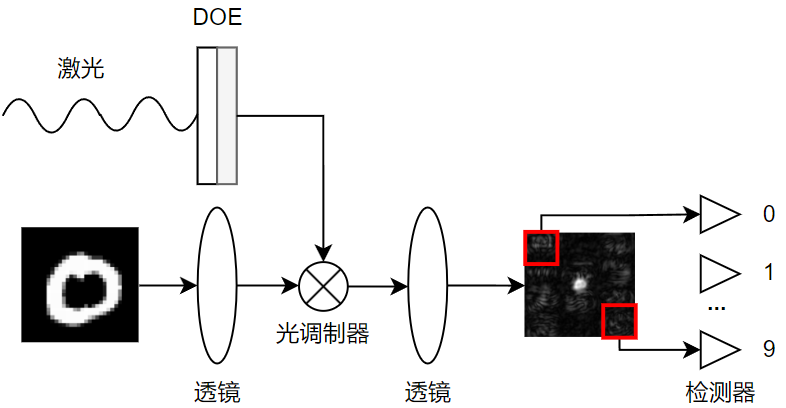
\includegraphics[width=0.95\textwidth]{pics/onn.png}
    \caption{光学神经网络模型}
    \label{fig:onn}
\end{figure}

如图\ref{fig:onn}所示,该光学神经网络的硬件部分包括透镜、DOE器件、光调制器、检测器等,可以实现对图像的处理。其中透镜负责傅立叶变换和逆傅立叶变换,DOE器件负责点光源转换,光调制器负责频谱图与高度图的点乘操作。最后,检测器负责接收处理后的图像,对每个区域的光强进行检测,实现对图像的分类任务。

在完成特征提取后,需要对特征图进行分类操作。传统的神经网络模型通常使用全连接层进行分类,而光学神经网络模型则可以将特征图划分为多个区域,计算每个区域的平均值作为概率分布。本实验中通过计算机模拟了这一过程,代码如下所示:

\newpage

\begin{lstlisting}[style=Python]
def center(a_tensor):
    squeeze_atensor = torch.squeeze(a_tensor)
    begin = end = 15
    center_tensor = squeeze_atensor[:, begin:-end, begin:-end]
    return torch.unsqueeze(center_tensor, -1)

def img_split(img):
    splitted_1d = torch.stack(torch.chunk(img, 4, dim=1), 0)
    splitted = torch.concat(torch.chunk(splitted_1d, 3, dim=3), 0)
    result = torch.stack(
        (center(splitted[0]), center(splitted[1]), center(splitted[2]),
         center(splitted[3]), center(splitted[5]), center(splitted[6]),
         center(splitted[8]), center(splitted[9]), center(splitted[10]),
         center(splitted[11])), 0)
    result = result.mean(dim=(2,3,4))
    result = torch.transpose(result, 0, 1)
    return result
\end{lstlisting}

上述\texttt{img\_split}函数实现了特征图的划分和分类操作,将图像在高度维度上拆分为4个区域,对于每个区域再在宽度维度上拆分为3个区域,总共得到12个区域,再选取除中间两个区域以外的10个区域。然后,通过\texttt{center}函数计算每个区域的中心部分,最后计算每个区域的平均值,得到一个长度为10的向量,作为分类的概率分布。

% 绘制示意图
% 子图1:首先绘制4x3网格,左上角为0,左下角为2,右下角为11
% 子图2:绘制1x10网格,序号分别为0、1、2、3、5、6、8、9、10、11,并在每个格子中心画一个红框
\begin{figure}[H]
    \centering
    \subfloat[特征图划分]{
        \resizebox{0.23\textwidth}{!}{
        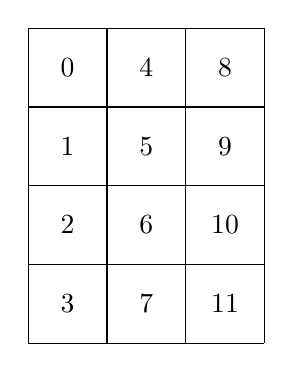
\begin{tikzpicture}
            \draw[step=1cm] (0,0) grid (3, 4);
            \node at (0.5, 3.5) {0};
            \node at (0.5, 2.5) {1};
            \node at (0.5, 1.5) {2};
            \node at (0.5, 0.5) {3};
            \node at (1.5, 3.5) {4};
            \node at (1.5, 2.5) {5};
            \node at (1.5, 1.5) {6};
            \node at (1.5, 0.5) {7};
            \node at (2.5, 3.5) {8};
            \node at (2.5, 2.5) {9};
            \node at (2.5, 1.5) {10};
            \node at (2.5, 0.5) {11};
        \end{tikzpicture}
        }
    }
    \subfloat[选择区域]{
        \resizebox{0.70\textwidth}{!}{
        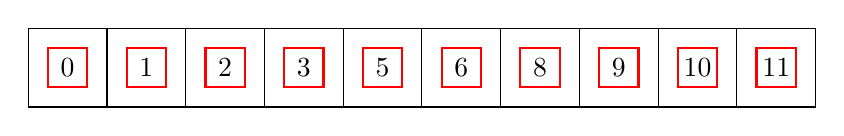
\begin{tikzpicture}
            \draw[step=1cm] (0,0) grid (10,1);
            \node at (0.5, 0.5) {0};
            \node at (1.5, 0.5) {1};
            \node at (2.5, 0.5) {2};
            \node at (3.5, 0.5) {3};
            \node at (4.5, 0.5) {5};
            \node at (5.5, 0.5) {6};
            \node at (6.5, 0.5) {8};
            \node at (7.5, 0.5) {9};
            \node at (8.5, 0.5) {10};
            \node at (9.5, 0.5) {11};

            \draw[red, thick] (0.25, 0.25) rectangle (0.75, 0.75);
            \draw[red, thick] (1.25, 0.25) rectangle (1.75, 0.75);
            \draw[red, thick] (2.25, 0.25) rectangle (2.75, 0.75);
            \draw[red, thick] (3.25, 0.25) rectangle (3.75, 0.75);
            \draw[red, thick] (4.25, 0.25) rectangle (4.75, 0.75);
            \draw[red, thick] (5.25, 0.25) rectangle (5.75, 0.75);
            \draw[red, thick] (6.25, 0.25) rectangle (6.75, 0.75);
            \draw[red, thick] (7.25, 0.25) rectangle (7.75, 0.75);
            \draw[red, thick] (8.25, 0.25) rectangle (8.75, 0.75);
            \draw[red, thick] (9.25, 0.25) rectangle (9.75, 0.75);
        \end{tikzpicture}
        }
    }
    \caption{特征图划分和分类}
    \label{fig:feature_split}
\end{figure}

如图\ref{fig:feature_split}所示,首先将特征图划分为3x4的网格,然后选择除中间两个区域以外的10个区域,选择每个区域中心标红部分计算平均值,得到一个长度为10的向量,作为分类的概率分布。

图\ref{fig:visualize}展示了特征图的可视化结果。可以看出,不同数字在不同网格区域的特征具有不同程度的激活,例如数字0在左上角区域有较强的激活,而数字9在右下角区域有较强的激活。这说明光学神经网络模型可以有效地提取图像的特征,实现图像分类任务。

% pics/viz0.png viz3.png viz6.png viz9.png
\begin{figure}[H]
    \centering
    \subfloat[数字0与特征图]{
        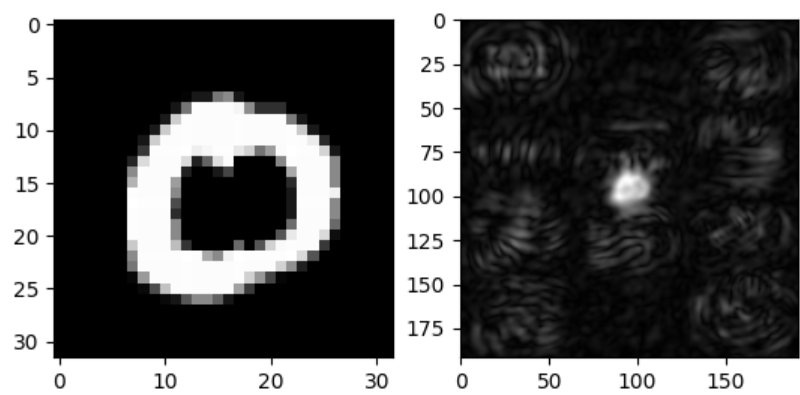
\includegraphics[width=0.45\textwidth]{pics/viz0.png}
    }
    \subfloat[数字3与特征图]{
        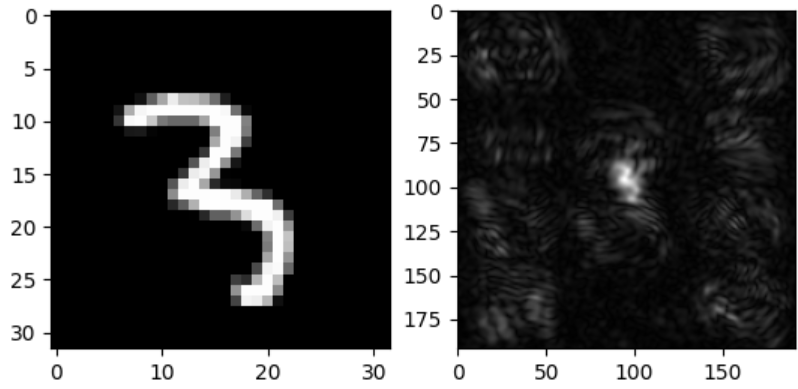
\includegraphics[width=0.45\textwidth]{pics/viz3.png}
    }\\
    \subfloat[数字6与特征图]{
        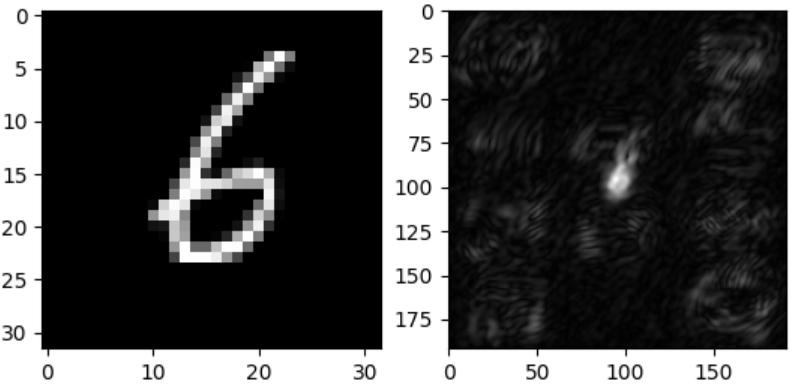
\includegraphics[width=0.45\textwidth]{pics/viz6.png}
    }
    \subfloat[数字9与特征图]{
        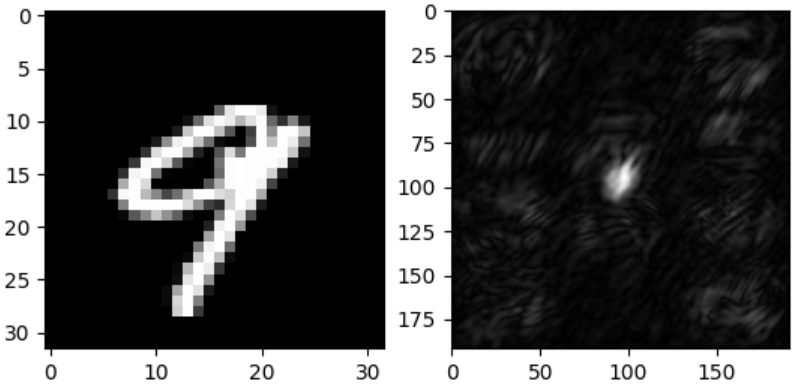
\includegraphics[width=0.45\textwidth]{pics/viz9.png}
    }
    \caption{特征图可视化}
    \label{fig:visualize}
\end{figure}

通过上述步骤,完成了光学神经网络的特征提取器和分类器的搭建,之后通过计算机模拟结构,对光学神经网络模型进行训练和测试。在MNIST数据集上,模型的准确率达到了94.9\%,表明光学神经网络模型可以进行有效的图像分类任务。
